\subsection{Pluvma}
\label{sec:specie-pluvma}

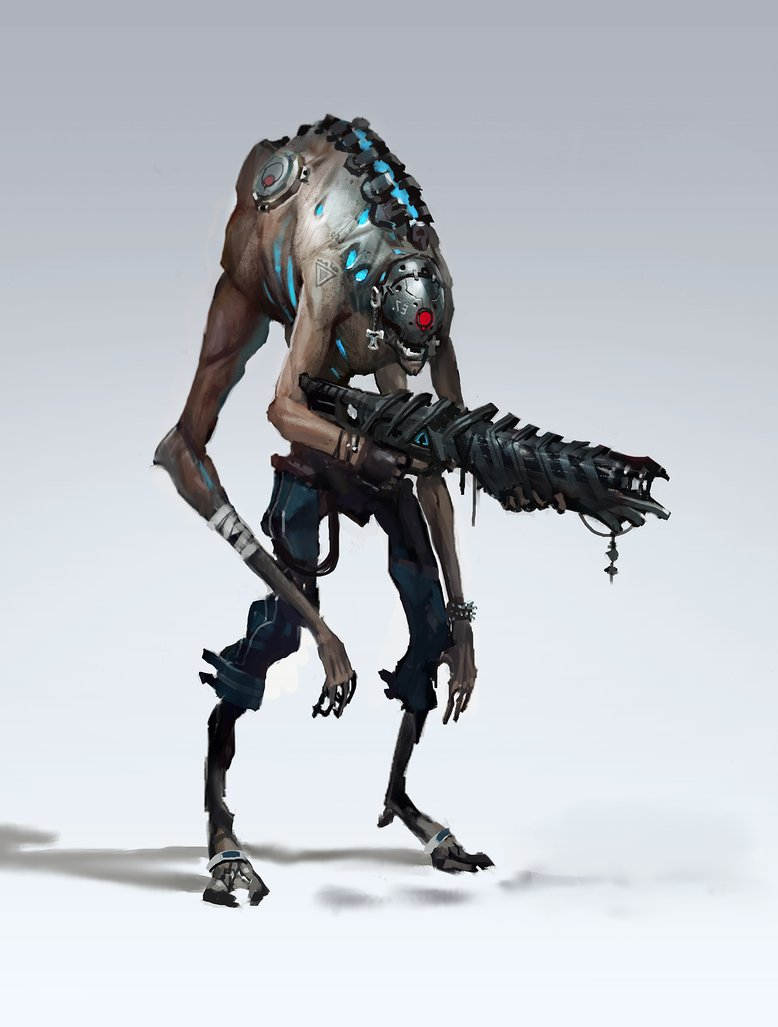
\includegraphics[width=\linewidth]{soldier_by_zoonoid-d4qf4cg}

\begin{redtable}{\linewidth}{@{}L{.35}@{}L{.65}@{}}
  \textbf{Singular} & Pluv\\
  \textbf{Plural} & Pluvma\\
  \textbf{Height} & 150-200cm\\
  \textbf{Weight} & 55-115kg\\
  \textbf{Gender Ratio} & 80\% Male / 20\% Female\\
  \textbf{Reproduction} & Viviparity (Live birth)\\
  \textbf{Maturity} & 20 years\\
  \textbf{Diet} & Omnivore\\
  \textbf{Homeworld} & Reistus (Lost)\\
\end{redtable}

The Pluvma are a multi-limbed alien species that is considered curious and quirky. They are as tall and weigh about the same as a human, with most of their mass located on the top half of their body. They have four arms that are each as functional as a humans, allowing a Pluvmian to manipulate more things at once. Even with the extra arms, the Pluvma only have a single eye which means they have trouble with depth perception.

Females in Pluvma society are generally rare, so males generally have to stand out from the pack to attract the opposite sex. This has resulted in Pluvmian society revolving around discovering something new and different, and if the Pluvmian male cannot they default to \textit{being} something new and different. It is because of this that no two Pluvmian males will ever purposely act alike.

To create a Pluvmian character, please refer to the \textit{\hyperref[sec:rules-creation]{Character creation section}}

\textbf{Pluvmian Male Names:}

Abbagan, Buckia, Bundamerrie, Chiridie, Coolanyarra, Doontah, Coombooloo, Jiwabiddy, Kagageerra, Mongah, Moolyal, Morangoril, Nangerow, Narga, Painbiddy, Tumbunna, Unjung, Wobbing, Yabongona, Yulla

\textbf{Pluvmian Female Names:}

Bobong, Booyo, Bringie, Chacca, Cookal, Dongo, Hynman, Inyah, Junman, Kurra, Milla, Noggo, Noothy, Nowen, Ronga, Tubar, Ula, Wisney, Woodya, Yanyea

\textbf{Secondary Names:}

Anakaus, Bisahalani, Degotoga, Espowyes, Gawonish, Harkahome, Hesutuvito, Keezheekoni, Kusinut, Lenmana, Mantotohpa, Matchitehew, Melkedoodum, Ocunnohurst, Ojinjintka, Quahneah, Sikyatavo, Taregan, Wawetseka, Wokaihwoko
